\tcbset{CajaconCapas/.style={%
		colback=yellow!2, % Color de fondo
		enlarge top by=1cm, % Espacio arriba (por la imagen)
		enhanced, % Habilitar código TikZ
		breakable, % habilitado el quiebre de caja
		boxrule=0pt, % sin borde (0pt)
		top=7mm, % espacio vertical del borde al texto = 7mm
		drop fuzzy shadow, % sombra
		overlay unbroken = {
			% Barra vertical
			% xshift = corrimiento horizontal
			% yshift = corrimiento vertical
			\draw[color=blue!80!yellow,line width =3pt]
			([xshift=2pt] frame.north west)--([xshift=2pt] frame.south west);
			% Barra horizontal
			\draw[color=blue!80!yellow,line width =1pt]
			( frame.north west)--(frame.north east);
			% Caja de imagen
			\node[rectangle] at ([xshift=1cm,yshift=0.45cm]frame.north west)
			{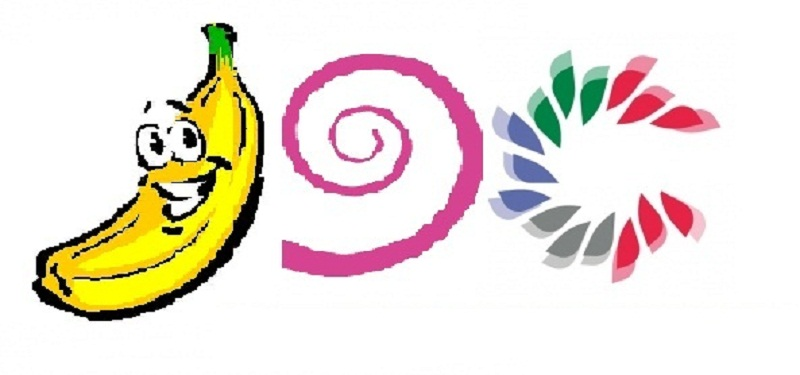
\includegraphics[scale=0.1]{images/caracol}};
			% Caja de descripción
			% minimum width = tamaño mínimo del rectángulo
			\node[rectangle, draw=DeepSkyBlue1, fill=DeepSkyBlue1,
			font=\LARGE\bfseries, text=white, rounded corners=8pt,minimum width =3cm
			,
			inner sep=1mm,anchor=north west] at
			([xshift=4cm,yshift=0.3cm]frame.north west){Ejercicios};
		},
		overlay first = {% capa superior
			% Barra vertical
			\draw[color=red!80!yellow,line width =3pt]
			([xshift=2pt] frame.north west)--([xshift=2pt] frame.south west);
			% Barra horizontal
			\draw[color=red!80!yellow,line width =1pt]
			( frame.north west)--(frame.north east);
			% Caja de imagen
			\node[rectangle] at ([xshift=1cm,yshift=0.45cm]frame.north west)
			{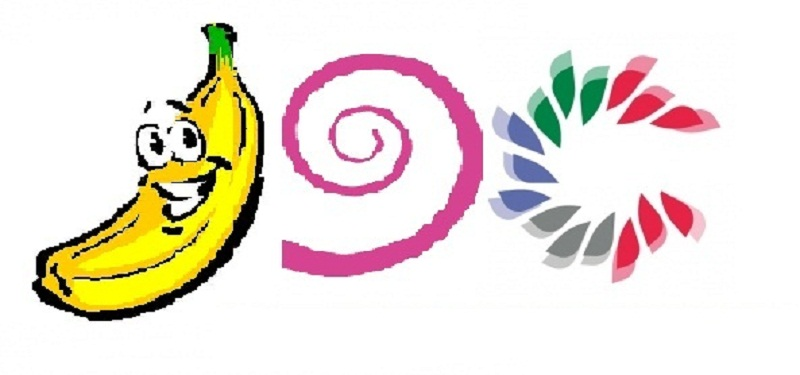
\includegraphics[scale=0.1]{images/caracol}};
			% Caja de descripción
			% minimum width = tamaño mínimo del rectángulo
			\node[rectangle, draw=DeepSkyBlue1, fill=DeepSkyBlue1,
			font=\LARGE\bfseries, text=white, rounded corners=8pt,minimum width =3cm
			,
			inner sep=1mm,anchor=north west] at
			([xshift=4cm,yshift=0.3cm]frame.north west){ Ejercicios};
		}, %First
		% Lo que permanece ante cambio de páginas
		overlay middle = { % Barra vertical
			\draw[color=red!80!yellow,line width =3pt]
			([xshift=2pt] frame.north west)--([xshift=2pt] frame.south west);
		},
		% Permanece la barra vertical
		overlay last={\draw[color=red!50!black!50,line width =3pt]
			([xshift=3pt] frame.north west)--([xshift=2pt] frame.south west);
		}
}}


